\chapter{Curvature and distant disks}\label{chapter:curvature-and-distant-disks}

In chapter \ref{chapter:digital-flow} we present the DCE algorithm and we remark that the choice of the ring number is of fundamental importance in order to derive a smooth flow. This observation lead us to ask if there is any relation between curvature and outer rings. In this appendix we give a positive answer for this question.

\section{Estimating curvature with outer disks}

Let $\mathcal{C}$ an oriented curve in the plane. We center disks $B_i$ and $B_o$ of radius $R + \epsilon$ and its centers aligned with the normal direction of the curve at some point $p \in \mathcal{C}$. Moreover, the distance from disks center to $p$ equals to $R$.

\begin{figure}
\center
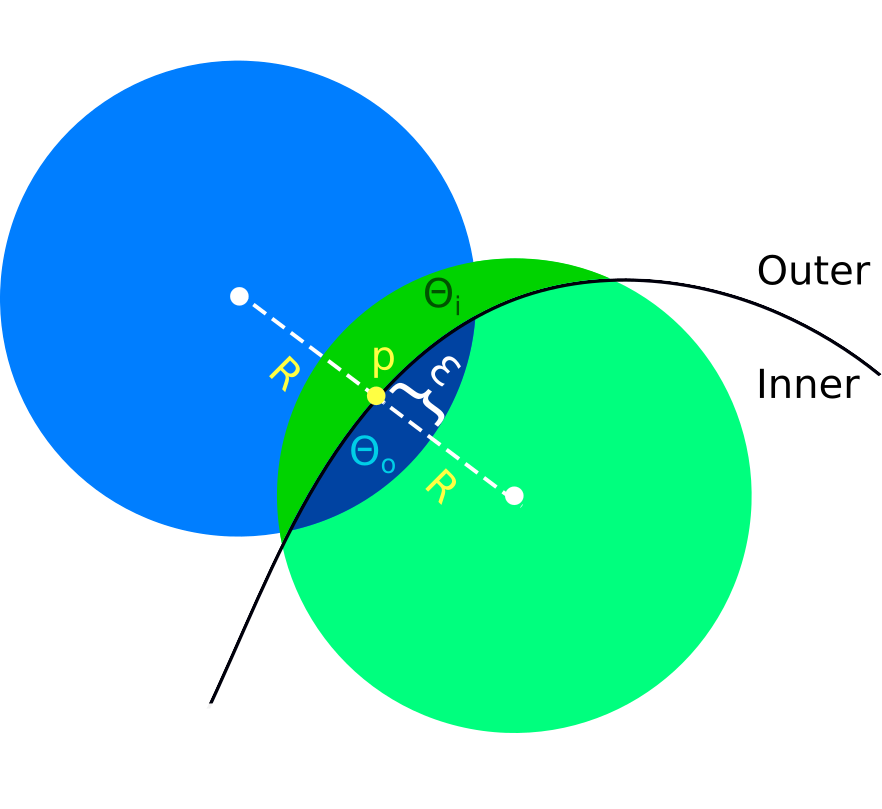
\includegraphics[scale=0.35]{figures/appendix-max-energy/r-separated-disks.png}
\caption{disks of radius $R+\epsilon$ distant $R$ units from $p\in \mathcal{C}$ in the normal direction.}
\label{fig:r-separated-disks}
\end{figure}

Let $\Theta_o (\Theta_i)$ to denote the intersection of $B_o(B_i)$ with the inner(outer) region of the curve. We define the function $g_R:\mathcal{R} \times \mathcal{C}\rightarrow \mathbb{R}$ as

\begin{align*}
	g_{R}(p) &= \Big( \Theta_i(p) - \Theta_o(p) \;\Big)^2.
\end{align*}

\begin{claim}{R-separated disks curvature}\label{claim:r-separated-disks}
 Let $\mathcal{C} \in \mathbb{R}^2$ be a curve such that for a point $p \in \mathcal{C}$ its curvature equals to $\kappa$. For $\epsilon=R/2$ and for sufficiently small values of $R$ and $\kappa$, we can approximate $g_R$ by


%\begin{align*}
%g_R(p) \approx & \frac{125}{144}R^6k^2 + \frac{625}{768}R^8k^4 + O(R^{10}\kappa^6)
%\end{align*} 

\begin{align*}
g_R(p) \approx & \frac{125}{144}R^6k^2 + O(R^{8}\kappa^4)
\end{align*} 

\end{claim}


\begin{proof} For every point $p$ in $C$, consider its Frenet frame formed by the tangent vector at $p$, $T(p)$ and the normal vector at $p$, $N(p)$. We assume the origin of the frame is at point $p$. Let $x$ be a variable in the axis defined by $T(p)$. Expanding $C(x)$ around the origin we obtain

\begin{align*}
	C(x) &= C(0) + \frac{dC}{dx}x + \frac{1}{2}\frac{d^2C}{dx^2}x^2 + O(x^3) \\
	&= \frac{\kappa}{2}x^2 + O(x^3).
\end{align*}

In other words, the second order approximation for the curve $C$ in the Frenet frame is the parabola $f(x) =  \kappa/2x^2$ passing at the origin. We are going to use this parabola to estimate $\Theta_o$ and $\Theta_i$.

We proceed by computing the intersection area $\Theta_o$.


\begin{figure}[h!]\label{fig:parabola-approx-ex}
\center
	\subfloat[\label{}]{%
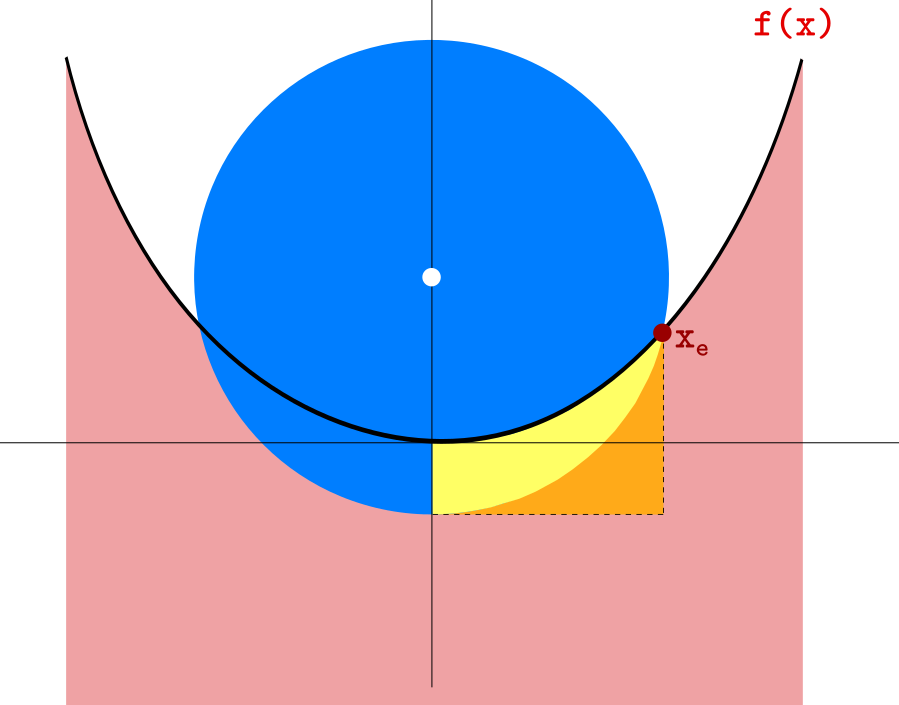
\includegraphics[scale=0.35]{figures/appendix-max-energy/parabola-approx-1.png}
	}\hspace{20pt}%
	\subfloat[\label{}]{%
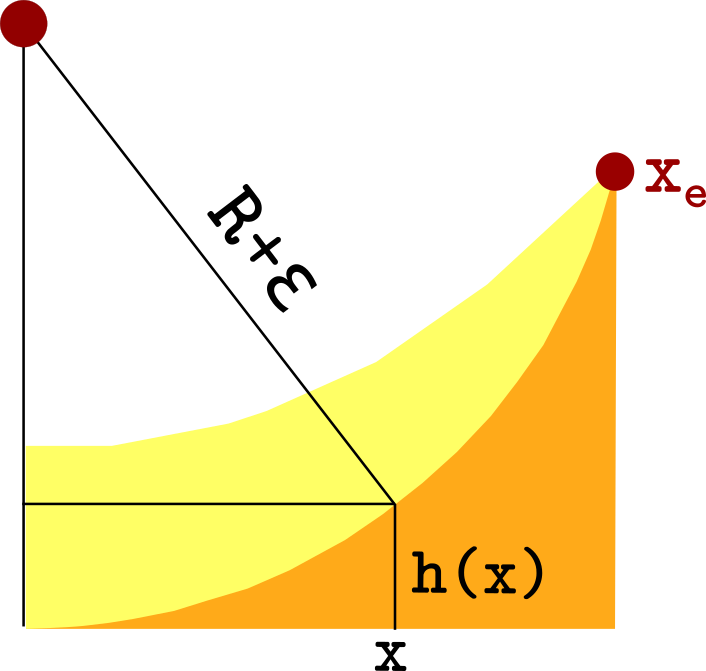
\includegraphics[scale=0.35]{figures/appendix-max-energy/parabola-approx-2.png}
	}
\caption{The yellow area equals $\Theta_o /2$, the same value of the area under the parabola from $x=0$ until $x=x_o$ minus the orange area $h(x)$.}
\end{figure}

\begin{align*}
	h(x) &= R+\epsilon - \sqrt{ (R+\epsilon)^2 - x^2}\\
	\Theta_o &= 2\int_0^{x_o}{f(x) + \epsilon - h(x)}\\
\end{align*}

To compute the intersection point $x_o$ of the parabola with the disk, we use again Pythagoras' theorem.

\begin{align*}
	(R+\epsilon)^2 &= (R-\frac{\kappa}{2}x_o^2)^2 + x_o^2\\
	0 &= \frac{\kappa^2}{4}x_o^4 + (1-R\kappa)x_o^2 + R^2 - (R+\epsilon)^2
\end{align*}

By setting $z_o=x_o^2$

\begin{align*}
\Delta_o &= (1-R\kappa)^2 + \kappa^2(2R\epsilon + \epsilon^2)\\
z_o &= \frac{2}{\kappa^2}(R\kappa-1 + \sqrt{\Delta_o})\\
x_o &= \frac{\sqrt{2}}{\kappa}\sqrt{R\kappa-1+\sqrt{\Delta_o}}
\end{align*}

We proceed similarly for the inner disk.


\begin{figure}[h!]\label{fig:parabola-approx-in}
\center
	\subfloat[\label{}]{%
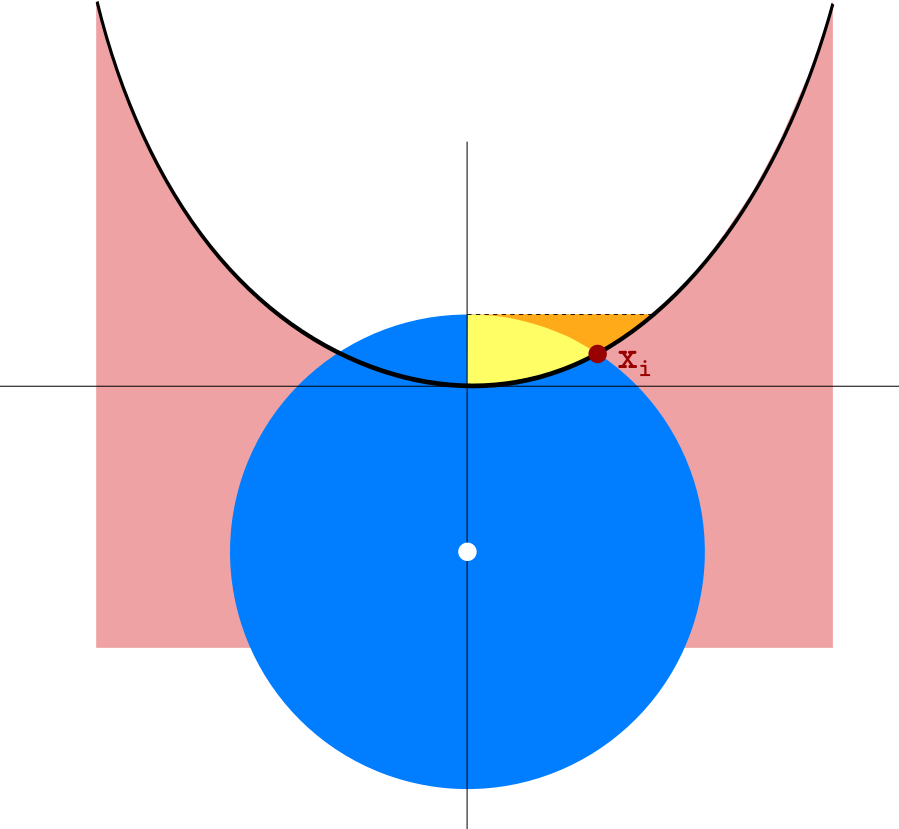
\includegraphics[scale=0.35]{figures/appendix-max-energy/parabola-approx-3.png}
	}\hspace{15pt}%
	\subfloat[\label{}]{%
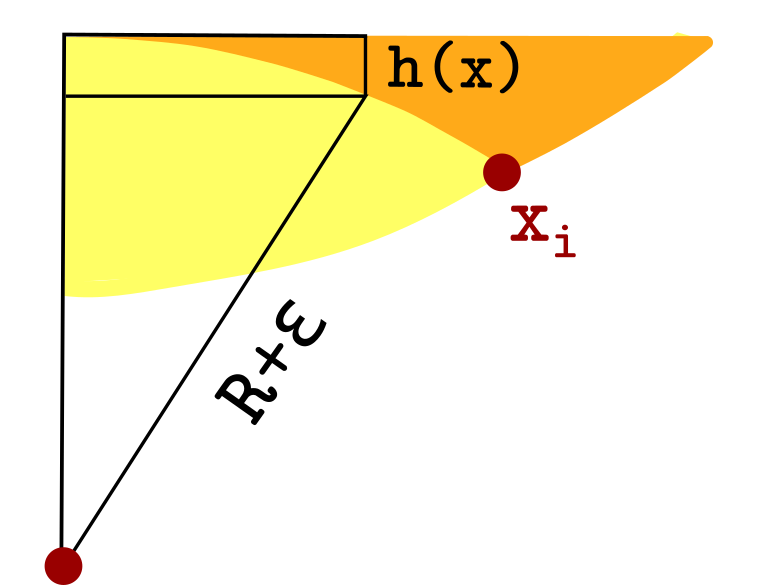
\includegraphics[scale=0.35]{figures/appendix-max-energy/parabola-approx-4.png}
	}
\caption{The yellow area corresponds to $\Theta_i$ and it equals the area between the parabola and the disk from $x=0$ until $x=x_i$.}
\end{figure}

\begin{align*}
	\Theta_i &= 2\int_{0}^{x_i}{\epsilon - f(x) - h(x)}	\end{align*}

The intersection point $x_i$ between the parabola and the inner disk is given by
	
\begin{align*}
	(R+\epsilon)^2 &= (R+\frac{\kappa}{2}x_o^2)^2 + x_i^2\\
	0 &= \frac{\kappa^2}{4}x_i^4 + (1+R\kappa)x_i^2 + R^2 - (R+\epsilon)^2	\\
\Delta_i &= (1+R\kappa)^2 + \kappa^2(2R\epsilon + \epsilon^2)\\
x_i &= \frac{\sqrt{2}}{\kappa}\sqrt{-R\kappa-1+\sqrt{\Delta_i}}.
\end{align*}

The claimed approximation is obtained by expanding $g_R$ with its  6th order Taylor series around $\kappa=0,R=0$.
\end{proof}

Therefore, the squared curvature at point $p$ can be estimated as

\begin{align*}
	\hat{\kappa}_{R-sep} ^2 = \frac{144}{125R^6}g_R(p) .
\end{align*}

\section{Experimental validation}

We check if $g_{\epsilon,p}$ can be used as squared curvature estimator. It seems that in order to achieve higher precision we need a large radius and a small $\epsilon$.

